\documentclass[11pt,a4paper]{article}
\usepackage[T1]{fontenc}
\usepackage[utf8]{inputenc}
\usepackage[magyar]{babel}
\usepackage{lmodern}
\usepackage{amsmath}
\usepackage{enumitem}
\usepackage{tikz}
\usetikzlibrary{arrows.meta}
\usepackage[a4paper,margin=2cm]{geometry}

\pagestyle{empty}
\setlength{\parindent}{0pt}
\setlist[enumerate,1]{label=\textbf{\arabic*.}, leftmargin=*, itemsep=9pt, topsep=3pt}

\begin{document}

\begin{center}
  {\large\bfseries Hőerőgépek, hatásfok, II.~főtétel -- megoldókulcs}\\[3pt]
  \fbox{\parbox{0.8\textwidth}{\centering
    $\Delta E = Q + W$, ahol $W$ a gázon végzett munka.\\
    A hatásfok nevezőjében \textbf{csak} a felvett hő szerepel.}}
\end{center}

\begin{enumerate}
\item $W_\text{h} = Q_\text{be} - |Q_\text{le}| = 800~\text{J} - 500~\text{J} = 300~\text{J}$,
  és $\eta = \dfrac{300~\text{J}}{800~\text{J}} = 0{,}375 = 37{,}5\%$.
  (Egy teljes ciklusban $\Delta E = 0$, ezért a hők különbsége a hasznos munka.)

\item
\begin{minipage}[t]{0.66\linewidth}
  Ellenkező irányban ($A\to D\to C\to B\to A$, az óramutatóval ellentétesen) a gép
  \textbf{hűtőgép / hőszivattyú} lesz. A vázlaton \textbf{mindhárom nyíl megfordul}:
  a gép a hideg tartályból $Q_\text{fel}$ hőt vesz fel, kívülről $W$ munkát kap, és a meleg
  tartálynak $Q_\text{le}$ hőt ad le. Energiamérleg: $Q_\text{le} = Q_\text{fel} + W$.

  A hő tehát a hidegebb helyről a melegebb felé áramlik, ehhez kívülről \textbf{munkát}
  kell befektetni (kompresszor, elektromos energia).

  Számokkal ($p_0V_0$ egységben, az előző órai értékek ellentettjei): felvett hő
  $\tfrac52 + 3 = \tfrac{11}{2}$ ($A\to D$, $D\to C$), leadott hő $5 + \tfrac32 =
  \tfrac{13}{2}$ ($C\to B$, $B\to A$), befektetett munka $W = +1$.

  \emph{Példák:} hűtőszekrény (a belsejéből a konyhába viszi a hőt), klíma,
  hőszivattyús fűtés.
\end{minipage}\hfill
\begin{minipage}[t]{0.30\linewidth}\vspace{0pt}\centering
  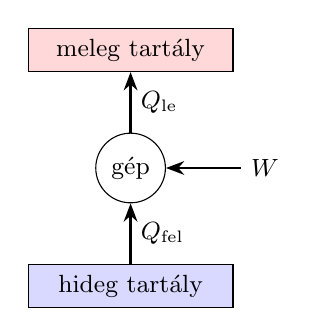
\begin{tikzpicture}[font=\small]
    \node[draw,fill=red!15,minimum width=2.6cm,minimum height=0.55cm] (M) at (0,1.5) {meleg tartály};
    \node[draw,circle,minimum size=0.75cm] (G) at (0,0) {gép};
    \node[draw,fill=blue!15,minimum width=2.6cm,minimum height=0.55cm] (H) at (0,-1.5) {hideg tartály};
    \draw[-{Stealth},thick] (G) -- node[right] {$Q_\text{le}$} (M);
    \draw[-{Stealth},thick] (H) -- node[right] {$Q_\text{fel}$} (G);
    \draw[-{Stealth},thick] (1.4,0) node[right] {$W$} -- (G);
  \end{tikzpicture}
\end{minipage}

\item A többi 3~kJ a \textbf{hideg környezetből} származik (külső levegő, talaj vagy
  talajvíz): $Q_\text{le,ház} = W + Q_\text{fel,kint} = 1~\text{kJ} + 3~\text{kJ}$.
  \begin{itemize}[nosep,leftmargin=1.5em]
    \item \textbf{I.~főtétel:} az energia megmarad, $1 + 3 = 4$~kJ, semmi sem keletkezik a
      semmiből. A 4-es arány nem ,,400\%-os hatásfok'', hanem jósági (fűtési) tényező.
    \item \textbf{II.~főtétel:} a hő magától nem megy hidegről melegre, de \emph{munka
      befektetése árán} igen. A II.~főtétel csak azt tiltja, hogy ez egyéb változás
      nélkül, magától történjen.
  \end{itemize}
  (Kiegészítés: $20\,^\circ$C belső és $0\,^\circ$C külső hőmérséklet között az elméleti
  maximum $T_\text{m}/(T_\text{m}-T_\text{h}) = 293/20 \approx 15$, a 4 tehát bőven
  megengedett.)

\item \textbf{a)} \emph{Magától végbemegy:} a hő a melegebb testről a hidegebbre áramlik,
  amíg a hőmérsékletek ki nem egyenlítődnek.

  \textbf{b)} \emph{Magától nem megy végbe:} a hő magától nem áramlik a hidegebb testről
  (szoba) a melegebbre (kávé). Az I.~főtételt ez nem sértené (a kávé annyi energiát kapna,
  amennyit a szoba lead), a II.~főtételt viszont igen.

  \textbf{c)} \emph{Magától nem megy végbe:} az I.~főtétel ezt sem tiltaná, ha a labda
  belső energiája éppen $mgh$-val csökken. A II.~főtétel viszont tiltja: a labda
  rendezetlen hőmozgásának energiáját kellene maradéktalanul rendezett mozgássá
  (mechanikai energiává) alakítani, egyéb változás nélkül. A fordított folyamat (a labda
  leesik, a pattogás után megáll és kissé felmelegszik) magától végbemegy.

\item \textbf{a)} \textbf{Elsőfajú perpetuum mobile:} olyan gép, amely energiabefektetés
  nélkül végez munkát, vagyis a semmiből termel energiát. Az \textbf{I.~főtételt}
  (energiamegmaradás) sértené.
  \textbf{Másodfajú perpetuum mobile:} olyan periodikusan működő gép, amely egyetlen
  hőtartályból felvett hőt teljes egészében munkává alakít. Az energia megmaradna, de a
  \textbf{II.~főtételt} sértené.

  \textbf{b)}
  \begin{enumerate}[label=(\arabic*),leftmargin=2em,itemsep=3pt,topsep=2pt]
    \item \textbf{Elsőfajú.} Egy teljes fordulat után a kerék ugyanabba az állapotba kerül
      vissza, a nehézségi erő munkája egy teljes körre nulla, így munkát nem nyerhetünk
      belőle. (A kihajló oldalon a súlyok messzebb vannak a tengelytől, de kevesebb van
      belőlük, a forgatónyomatékok kiegyenlítik egymást; a súrlódás miatt a kerék le is áll.)
    \item \textbf{Elsőfajú.} Sem a motor, sem a generátor hatásfoka nem 100\%: a generátor
      még a motor működtetéséhez szükséges energiát sem tudja visszaadni, nemhogy egy
      izzót is táplálni. A ,,felesleg'' a semmiből keletkezne.
    \item \textbf{Másodfajú.} Az energia megmaradna (a víz lehűl, a hajó munkát végez), de
      a hajó egyetlen tartályból (a tengerből) venne fel hőt, és azt teljesen munkává
      alakítaná. A tenger óriási belső energiája nem segít: munkát csak két különböző
      hőmérsékletű tartály között nyerhetünk, a hajónak pedig nincs hidegebb tartálya,
      ahová a hő egy részét leadhatná.
    \item \textbf{Működhet}, mert két különböző hőmérsékletű tartály között dolgozik.
      $\eta_\text{max} = 1 - \dfrac{278~\text{K}}{298~\text{K}} = \dfrac{20}{298} \approx
      6{,}7\%$. Valóban léteznek ilyen kísérleti erőművek (OTEC); a gyakorlati hatásfok
      ennél is kisebb, és a víz szivattyúzása is energiát igényel.
  \end{enumerate}

  \textbf{c)} A lehűlő és felugró labda a környezetétől elszigetelt test hőjét alakítaná
  teljes egészében munkává (helyzeti energiává), egyéb változás nélkül. Ez éppen a
  másodfajú perpetuum mobile működési elve: ha a labda így viselkedne, ilyen gépet is
  építhetnénk.

\item \textbf{Mintaválasz:}
  A hőerőgép periodikusan működő berendezés, amelyben egy munkaközeg (pl.\ gáz vagy gőz)
  körfolyamatot végez. A ciklus egy részében a munkaközeg a meleg tartálytól (pl.\ égő
  üzemanyagtól) $Q_\text{be}$ hőt vesz fel, kitágul, és közben munkát végez a
  környezetén. Hogy a gép újra és újra működhessen, a munkaközegnek vissza kell térnie a
  kiinduló állapotába, ezért össze kell nyomni. Ha ezt ugyanazon a magas hőmérsékleten
  tennénk, éppen annyi munkát kellene befektetnünk, amennyit a táguláskor nyertünk, és nem
  maradna hasznos munka. Ezért a munkaközeget lehűtjük, és alacsonyabb hőmérsékleten,
  kisebb nyomáson nyomjuk össze, miközben $Q_\text{le}$ hőt ad át a hideg tartálynak
  (pl.\ a környezet levegőjének vagy a hűtővíznek). Mivel egy teljes ciklus után a belső
  energia nem változik, az I.~főtétel szerint a hasznos munka
  $W_\text{h} = Q_\text{be} - |Q_\text{le}|$. A II.~főtétel szerint a felvett hőt nem
  lehet teljes egészében munkává alakítani, ezért a hideg tartály nélkülözhetetlen, és a
  hatásfok $\eta = W_\text{h}/Q_\text{be}$ mindig kisebb 1-nél.

  \medskip
  \textbf{Pontozási szempontok} (ami nélkül nem teljes a válasz):
  \begin{itemize}[nosep,leftmargin=1.5em]
    \item munkaközeg, körfolyamat, periodikus működés;
    \item hőfelvétel a meleg tartályból és munkavégzés (tágulás);
    \item a munkaközeg visszajuttatása a kiinduló állapotba, ehhez hűtés és hőleadás a
      hideg tartálynak;
    \item energiamérleg: $\Delta E = 0$ egy ciklusra, $W_\text{h} = Q_\text{be} -
      |Q_\text{le}|$;
    \item a II.~főtétel megemlítése: a hő nem alakítható teljesen munkává, $\eta < 1$;
    \item összefüggő, szabatos szöveg (nem felsorolás!).
  \end{itemize}
\end{enumerate}

\end{document}
